\chapter{Developing for Android}
\label{chap:android}

Android, Inc\@. was founded in October in 2003 by Andy Rubin, Rich Miner, Nick Sears, and Chris White. 
At first, the company planned to develop an operating system for digital cameras % but when they realised that the market is not large enough,
but ultimately % they decided to change their intentions and 
decided to focus on smartphones instead. % operating system.
% That time, the Apple's iPhone was not released yet. 
% The rival mobile phones operating systems were Symbian and Windows Mobile.
% After four years with the financial aid of Google, Android was revealed.
HTC Dream, the first phone with the Android operating system, was sold in autumn 2008.
Majority of Android's code is released under a free license. 
This allows developers to modify and (with certain exceptions) freely distribute the software.
Due to this, Android became the most popular operating system for smartphones.
In this chapter, we introduce this system from programmer's perspective and give a brief description of how to implement an Android application.
The purpose of the chapter is to highlight the main architectural differences between Android and conventional desktop platforms rather then providing a complete programer's manual. 

\section{Introduction to the Android development}

% Android is a product of \term{The Open Handset Alliance}, which develops open standards for mobile devices and is led by Google.
The Android platform is a layered environment built on the foundation of the Linux kernel.
It includes a user interface library featuring various types of elements (views, windows, display boxes, lists, etc.),  
an embedded web browser, and support for OpenGL ES.
Most Android-powered devices have built-in sensors to measure, e.g., motion, orientation or temperature. 
These include an accelerometer, a gyroscope or a barometer.
It also provides an array of connectivity options, for example Wi-Fi, Bluetooth or cellular data.
A built-in camera support is also included and most Android handsets indeed feature a camera. 
% In an effort to improve graphics, the Android platform supports an environment for 2D and 3D graphics development including OpenGL library.
The data storage support is provided by SQLite, a relational database management system in the form of a library implementing self-contained and server-less SQL database engine.
 
Linux kernel, the first architectural layer of the platform, is used for memory and process management, device drivers, and networking.
Above this, we have the native libraries, which include graphics support, media codecs, SQLite, and WebKit.
These are written in C or C++ and called through a Java interface.
The actual applications are running on the Dalvik Virtual Machine (DVM), an implementation of the Java Virtual Machine optimized for low processing power and memory resources.
% We should note that the virtual machine applications are running within is not Java virtual machine, but Dalvik Virtual machine.
The Android Runtime Layer consists of this DVM and the core Java libraries. 

The next level is the Application Framework, which manages functions fundamental to running applications.
Its major part is formed by the Activity Manager (managing the life cycle of the applications) and various Content Providers (managing data sharing between the applications).
Other notable parts are the Telephony Manager (handling voice calls), the Location Manager (specifying location using GPS or cell tower) and the Resource Manager.
The final layer is formed by the individual applications.
Some of them are preinstalled and provided by Google while the rest are third party applications created by the community.
The structure of the system is illustrated in Figure \ref{fig:architecture} below.
\begin{figure}[h!]
    \centering{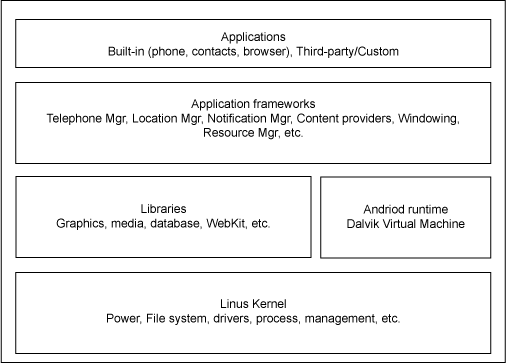
\includegraphics[width=80mm]{img/software_layers.png}}
    \caption{The architecture of the system.} 
    \label{fig:architecture}
\end{figure}

Android applications are written in the Java programming language and run within an instance of the Dalvik Virtual Machine.
A key part of the application is the AndroidManifest\@.xml file containing installation meta-data, including the necessary permissions.
An example of such permission is the ability to use the phone's camera or to access the Internet.
\begin{figure}[h!]
    \centering{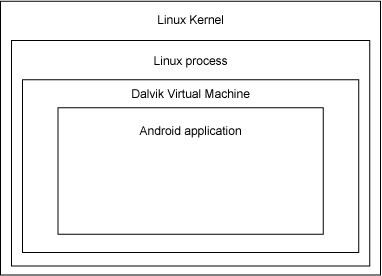
\includegraphics[width=80mm]{img/dalvik.png}}
    \caption{A typical Android application runs within an instance of the Dalvik Virtual Machine.}
\end{figure}

The tools required for the development of an Android application are the Android Software Development Kit (SDK)\footnote{\url{http://developer.android.com/sdk/}} and a Java IDE, such as Eclipse\footnote{\url{http://www.eclipse.org}} or the Android Studio\footnote{\url{http://developer.android.com/sdk/installing/studio.html}} based on IntelliJ IDEA. 
The Android SDK contains an Eclipse plugin supporting Android developement, documentation, sample code, and various tools, such as the Android Debug Bridge used by the programmer to communicate with an application running on a device or an emulator. 
% % \item The Android SDK is provided as \@.zip file including Java archive file containing all necessary classes to build an application (android\@.jar),
% the SDK documentation, a directory with sample code, Android Debug Bridge and other tools needed to build an application.

% TODO: tohle pripadne pridejme az ten text bude vyladenejsi: In the rest of this chapter we describe some of the implementational parts of the application development. 

\section{Application components}

Compared to the situation on the majority of conventional platforms, Android interacts with the running applications in a much closer manner. 
Actually, the system expects a certain specific architectural structure of the application expressed using concepts from object oriented programming. 
A typical Android application is be decomposed into several classes, each being a descendant of a particular class provided by the SDK. 
Through this, requirements on what and how the application's class has to implement are imposed. 
This approach allows, e.g., sophisticated interaction between different applications running on the same phone. 
For example, one application can use a list of contacts maintained by another application without the developers of the latter having to set up any protocols or data exports -- they only need to obey the software development principles of the platform. 
Thanks to this, the user data are seamlessly protected from an unauthorised access by the system through the principle of least privilege. 
In the above-mentioned example, the access to the list of contacts would not be granted unless it is listed in the accessing application's manifest file and this requirement has been authorized by the user. 
Since these properties of the platform are rather unique, we devote this section to discuss them. 

An Android application is built from several components typically belonging to one of the following groups: 
\begin{itemize}
\item{activities,}
\item{services,}
\item{content providers, etc.}
\end{itemize}

\term{An activity} can be thought of as a UI screen providing elements such as views, lists, buttons, labels, etc. along with the implementation of their functionality.
The layout of an activity and the widgets placed in the window is described in a separate XML file. 
Most applications consist of more than one activity with one being designated as the main one.
Although the activities form one application, they are all independent from each other.
If another application has a permission to do so, it can start an activity of a different app.
From the developer's perspective, activities are represented by classes descending from the Activity class defined in the SDK. 

\term{A service} is a component used to perform operations in the background.
For example, if the application needs to run a long-term computation, the user can switch to another application with the computation continues. 

\term{A content provider} manages sharing data across applications.
When the app is storing data, for example in the file system or an SQLite database, the content provider interface can be used to access or even modify the data from other applications. 

The platform utilizes additional classes of components besides the above-mentioned ones (e.g., broadcast receivers). 
However, we omit them for the sake of brevity. 

%%% docteno sem 
The interaction between various components and activities is facilitated by \term{intents.} 
An intent is a message to the system to invoke new activity, service or broadcast.
% It is a component activating mechanism in Android.
The reader is referred to the Android SDK documentation for more information about activities, services, content provides, intents, etc. 

\section{Activity lifecycle}
\label{sec:lifecycle}

During its life cycle, an application switches between different application states.
Compared to desktop platforms, the programmer has only limited control over these state transitions.
On the desktop computer, the developer has a certain level of control over, e.g., minimizing or closing a window of an application or quitting the software. 
This cannot be affected on the discussed platform. 
The life cycle is a collection of functions the operating system executes on the application during its runtime. 

There are five stages of the life of an application:
\begin{itemize}
\item the starting state,
\item the running state,
\item the paused state,
\item the stopped state,
\item and the destroyed state.
\end{itemize}

The starting state and the destroyed state are phases of the activity when it is not in the memory.
To launch the app, the main activity class's \emph{onCreate()} method is called and eventually the application transitions into the running state.
When in a running state, the application is actually on the screen visible to the user and handling all user interactions such as typing or touching the screen. 
An activity in this state has the highest priority for memory allocation in the activity stack.
It is killed by the operating system only in extreme situations.
This transition from starting to running state is the most expensive operation in terms of battery requirements.
That is also the reason why Android does not destroy every activity when it gets to the background, 
because it is probable that it is going to be used again. 

\begin{figure}[h!]
    \centering{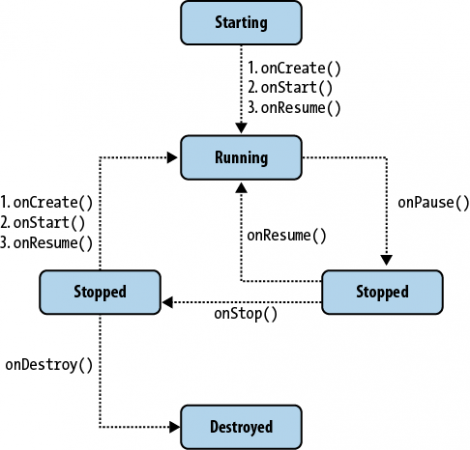
\includegraphics[width=80mm]{img/life_cycles.png}}
    \caption{Life cycle of an application.}
\end{figure}

The application is paused (in a paused state) when not interacting with user but is still visible on the screen.
This state does not occur very often, since most applications cover entire screen.
However, in the cases when the application is partly visible yet not interacting with the user, the pause state is utilized. 

When the application is not visible but still in memory, it is in a stopped state.
Then, it is easy to bring it up to the front again or it can be destroyed and thus removed from the memory.

\section{User interface}
\label{sec:ui}

All elements of the application's user interface are built using a hierarchy of \term{View} and \term{ViewGroup} objects.
The layout describing the visual structure of the \term{Views} is declared in a separate XML file.
Although not recommended, the user interface can be also declared explicitly in the source code. 
There are two principal layouting options: \term{LinearLayout} arranges the inner elements in a single row or a column,
while \term{RelativeLayout} positions the elements in relation to their parent or each other.

With the layout defined, the developer can then utilize the UI elements offered by the SDK, such as menus, action bars, \term{dialogs} or toasts.
There are several types of menus such as options menu or context menu. 
The options menu displays a collection of buttons when the user taps the menu button typically available on an Android device. 
From the Android version 3\@.0 higher, the options menu items are included in the action bar after touching the action overflow button. 
The context menu is a floating menu associated with a particular element in a view displayed after touching the element.

Action bars provide a way for navigating through the application's interface. 
The action bar is located at the top of an activity and can display the activity title, icon or other actions and items.
Some Android devices have a hardware action overflow button which opens the \term{options menu} at the bottom of an activity. 
\term{Action Bars} are superior to the \term{options menus} since an \term{action bar} is always visible while \term{options menu} shows only on the user request.

A \term{Dialog} is a small window informing the user about some action. 
Unlike \term{Toast} it usually requires the users action before continuing by confirmation or giving some additional information.
The \term{Toast} provides only feedback about some action in a small pop-up that disappears after a moment.

\section{Sensors}

Most Android devices have built-in motion, environmental and positional sensors.
Motion sensors are sensors measuring the rotation along three axes and give us an opportunity to detect motion, shaking or tilting of the device. 
Environmental sensors are applied for measuring temperature, illumination, or humidity.
Built-in magnetometers and orientation sensors provide information about the current position and/or orientation of a device and can be used in applications for GPS navigation or in mapping software. 
The sensor events are access using an instance of the \term{SensorManager} class.

\section{Data storage}

There are several possibilities for storing application data in Android. 
The internal storage is preferable when we do not want other applications to access them. 
The read and write operations are performed using instances of \term{FileInputStream} and \term{FileOutputStream}.

However, media files such as pictures, video files or audio records are expected to be shared and accessible from other applications.
In such a case, the external storage is utilized through methods of the \term{Environment} class.
The function \term{getExternalStoragePublicDirectory()} depending on the supplied argument returns the path of the root directory where we can write our data, for example: 
\begin{itemize}
\item{../Music/,}
\item{../Pictures/,}
\item{../Movies/,}
\item{../Download/,}
\item{etc.}
\end{itemize}
As an argument we pass the type of the directory we want to access, for example \term{Environment\@.DIRECTORY\_MUSIC}.

\section{Example} 

In this section, we illustrate the concepts from the above sections on an example application. 
As noted in the beginning of the chapter, this is not intended to be an all-encompassing description of creating an Android application. 
Rather, it is supposed to illustrate crucial parts the process. 

A user interface, discussed in Section \ref{sec:ui}, is typically specified using an XML file stored in the \term{/res/layout} directory.
Below is a simple example of such file: 

\begin{lstlisting}
    <?xml version="1.0" encoding="utf-8"?>
    <RelativeLayout xmlns:android="http://schemas.android.com/apk/res/android"
        xmlns:tools="http://schemas.android.com/tools"
        android:layout_width="match_parent"
        android:layout_height="match_parent">
    
        <org.opencv.android.NativeCameraView
            android:id="@+id/camera_view"
            android:layout_width="match_parent"
            android:layout_height="match_parent"/>
        
        <RelativeLayout
    	    android:layout_width="200dp"
    	    android:layout_height="match_parent"
    	    android:layout_margin="10dp"
    	    android:layout_centerInParent="true">
    	    
            <Button
    	        android:id="@+id/captureButton"
    	        android:layout_width="90dp"
    	        android:layout_height="90dp"
    	        android:layout_alignParentBottom="true"
    	        android:layout_centerHorizontal="true"
    	        android:background="@drawable/circle_button"
    	        android:onClick="callTakePicture"/>
            
            <Button
    	        android:id="@+id/startCapturingButton"
    	        android:layout_width="90dp"
    	        android:layout_height="90dp"
    	        android:layout_alignParentBottom="true"
    	        android:layout_centerHorizontal="true"
    	        android:background="@drawable/circle_button"
    	        android:onClick="start_stopAutoCapturing"
    	        android:visibility="invisible"/>
    	          
    	    <ToggleButton
    	        android:id="@+id/toggleAutoCaptureButton"
                    android:layout_width="wrap_content" 
                    android:layout_height="wrap_content" 
                    android:layout_alignParentTop="true"
                    android:layout_centerHorizontal="true"
    	        android:textOn="AutoCapture on"
    	        android:textOff="AutoCapture off"	    
    	        android:onClick="autoCaptureStateChanged"/>
    
    	    <TextView
    	        android:id="@+id/startCapturing_textView"
    	        android:layout_width="wrap_content"
    	        android:layout_height="wrap_content"
    	        android:layout_above="@+id/captureButton"
    	        android:layout_centerHorizontal="true"
    	        android:text="@string/startcapturing_text"
    	        android:visibility="invisible"/>
    
    	</RelativeLayout>
    	
    </RelativeLayout>
\end{lstlisting}

In our example, the root element is a \term{RelativeLayout} element which allows us to describe a relative position with respect to the parent. 
Inside the \term{RelativeLayout}, we find \term{org.opencv.android.NativeCameraView} which is an element of the OpenCV library used for camera view and another \term{RelativeLayout} with \term{Buttons}, a \term{ToggleButton} and a \term{TextView}.
All of the elements have their width and height specified by using the \term{android:layoutwidth} and \term{android:layoutwidth} attributes.
The value of these attributes can be \term{matchparent} or \term{wrapcontent} or a specific number of units.

It is possible to define a specific layout of an activity for a particular screen orientation through supplying an alternative XML file of the same name in the \term{res/layout-land} folder.

In the \term{src} folder, we have all the .java files representing activities or classes.
Every Android application has at least one ``main'' activity invoked by the system when the application is launched.
Due to the activity lifecycle (see Section \ref{sec:lifecycle}), it is necessary to implement the following methods:
\begin{itemize}
\item \term{onCreate()},
\item \term{onPause()},
\item \term{onResume()}.
\end{itemize}

Usually only the basic startup actions are completed in the \term{onCreate()} method, for example setting up the layout or initializing some of the class variables.
The implementation of the \term{onCreate()} method in the example below first invokes the ancestor's corresponding method, then initializes the layout using the \term{setContentView()} method and then performs some application specific processing. 
\begin{lstlisting}
    @Override
    public void onCreate(Bundle savedInstanceState) {
        super.onCreate(savedInstanceState);
        setContentView(R.layout.activity_gallery);
        
        adapter = new Adapter(this);
        ArrayList<GridImage> db_update = new ArrayList<GridImage>();
        for (String s : files) {
          ...
        }
        ...
    }
\end{lstlisting}
Depending on the needs of our application, we can add some code into the other overriding methods handling the activity lifecycle: 
\begin{lstlisting}
    @Override
    public void onPause(){
        super.onPause();
        ...
    }
  	
    @Override
    public void onResume(){
        super.onResume();
        ...
    }
\end{lstlisting}
To make the user interface interactive we need to assign functions to be executed when tapping on the individual elements.
This can be done either in the XML file by specifying the activity's method name in an attribute of the corresponding element: 
\begin{lstlisting}
    <Button  
      ...
      android:onClick="takePicture"
      ... />
\end{lstlisting}
Alternatively, the action can be assigned in the code:
\begin{lstlisting}
    Button my_button = (Button)findViewById(R.id.button);
    my_button.setOnClickListener( new View.OnClickListener() {
      ...    
    });
\end{lstlisting}









